\documentclass[11pt]{article}\usepackage[]{graphicx}\usepackage[]{color}
%% maxwidth is the original width if it is less than linewidth
%% otherwise use linewidth (to make sure the graphics do not exceed the margin)
\makeatletter
\def\maxwidth{ %
  \ifdim\Gin@nat@width>\linewidth
    \linewidth
  \else
    \Gin@nat@width
  \fi
}
\makeatother
\usepackage{pdfpages} 
\definecolor{fgcolor}{rgb}{0.345, 0.345, 0.345}
\newcommand{\hlnum}[1]{\textcolor[rgb]{0.686,0.059,0.569}{#1}}%
\newcommand{\hlstr}[1]{\textcolor[rgb]{0.192,0.494,0.8}{#1}}%
\newcommand{\hlcom}[1]{\textcolor[rgb]{0.678,0.584,0.686}{\textit{#1}}}%
\newcommand{\hlopt}[1]{\textcolor[rgb]{0,0,0}{#1}}%
\newcommand{\hlstd}[1]{\textcolor[rgb]{0.345,0.345,0.345}{#1}}%
\newcommand{\hlkwa}[1]{\textcolor[rgb]{0.161,0.373,0.58}{\textbf{#1}}}%
\newcommand{\hlkwb}[1]{\textcolor[rgb]{0.69,0.353,0.396}{#1}}%
\newcommand{\hlkwc}[1]{\textcolor[rgb]{0.333,0.667,0.333}{#1}}%
\newcommand{\hlkwd}[1]{\textcolor[rgb]{0.737,0.353,0.396}{\textbf{#1}}}%
\let\hlipl\hlkwb

\usepackage{ulem}

\usepackage{framed}
\makeatletter
\newenvironment{kframe}{%
 \def\at@end@of@kframe{}%
 \ifinner\ifhmode%
  \def\at@end@of@kframe{\end{minipage}}%
  \begin{minipage}{\columnwidth}%
 \fi\fi%
 \def\FrameCommand##1{\hskip\@totalleftmargin \hskip-\fboxsep
 \colorbox{shadecolor}{##1}\hskip-\fboxsep
     % There is no \\@totalrightmargin, so:
     \hskip-\linewidth \hskip-\@totalleftmargin \hskip\columnwidth}%
 \MakeFramed {\advance\hsize-\width
   \@totalleftmargin\z@ \linewidth\hsize
   \@setminipage}}%
 {\par\unskip\endMakeFramed%
 \at@end@of@kframe}
\makeatother

\definecolor{shadecolor}{rgb}{.97, .97, .97}
\definecolor{messagecolor}{rgb}{0, 0, 0}
\definecolor{warningcolor}{rgb}{1, 0, 1}
\definecolor{errorcolor}{rgb}{1, 0, 0}
\newenvironment{knitrout}{}{} % an empty environment to be redefined in TeX

\usepackage{alltt}
\usepackage{graphicx, fancyhdr}
\usepackage{amsmath, amsfonts}
\usepackage{color}
\usepackage{hyperref}

\newcommand{\blue}[1]{{\color{blue} #1}}

\setlength{\topmargin}{-.5 in} 
\setlength{\textheight}{9 in}
\setlength{\textwidth}{6.5 in} 
\setlength{\evensidemargin}{0 in}
\setlength{\oddsidemargin}{0 in} 
\setlength{\parindent}{0 in}
\newcommand{\ben}{\begin{enumerate}}
\newcommand{\een}{\end{enumerate}}


\lhead{STAT 305}
\chead{Homework \# 10} 
\rhead{Due Thursday, Dec. $5^{th}$ in the class}
\lfoot{Fall 2019} 
\cfoot{\thepage} 
\rfoot{} 
\renewcommand{\headrulewidth}{0.4pt} 
\renewcommand{\footrulewidth}{0.4pt} 

\def\Exp#1#2{\ensuremath{#1\times 10^{#2}}}
\def\Case#1#2#3#4{\left\{ \begin{tabular}{cc} #1 & #2 \phantom
{\Big|} \\ #3 & #4 \phantom{\Big|} \end{tabular} \right.}
\IfFileExists{upquote.sty}{\usepackage{upquote}}{}
\usepackage{Sweave}
\begin{document}
\Sconcordance{concordance:stat305_hw10.tex:stat305_hw10.Rnw:%
1 83 1 1 0 12 1 1 9 14 1 1 4 13 0 1 2 16 1 1 5 6 0 1 5 1 0 1 2 37 1}

\pagestyle{fancy} 

Show \textbf{all} of your work on this assignment and answer each question fully in the given context.\\

\emph{Note:}You can email your homework only if you cannot attend the class to submit your homewok. If you do so, email your homework by the noon of the due date. 


\emph{Please} staple your assignment!


\begin{enumerate}
	
    \item \textbf{[Ch. 6.1, Exercise 2, pg. 344]} We have a data set consisting of the aluminum contents of 26 bihourly samples of recycled PET plastic from a recycling facility. Those 26 measurements have $\overline{y} = 142.77$ ppm and $s \approx 98.2$ ppm. Use these facts to respond to the following.
    
      \begin{enumerate}
        \item Make a 90\% two-sided confidence interval for the mean aluminum content of such speciments over the whole study period.[5 pts]
        \item Make a 95\% two-sided confidence interval for the mean aluminum content of such speciments over the whole study period. How does this compare to your answer in part a)? [5 pts]
        \item Make a 90\% upper confidence bound for the mean aluminum content of such speciments over the whole study period. (Find a # such that $(\infty, \#)$ is a 90\% confidence interval.) How does this value compare to the upper endpoint of your interval from part a)? [5 pts]
        \item Make a 95\% upper confidence bound for the mean aluminum content of such speciments over the whole study period. (Find a # such that $(\infty, \#)$ is a 95\% confidence interval.) How does this value compare to the upper endpoint of your interval from part c)? [5 pts]
        \item Interpret your interval from a) for someone with little statistical background. [5 pts]
      \end{enumerate}
      
    \item \textbf{ [Ch 6.1, Exercise 4, pg. 344]} DuToit, Hansen, and Osborne measured the diameters of some no. 10 machine screws with two different calipers (digital and vernier scale). Part of their data are recorded here. Given in the small frequency table are the measurements obtained on 50 screws by one of the students using the digital calipers.



\begin{Schunk}
\begin{Soutput}
| Diameter| Frequency|
|--------:|---------:|
|     4.52|         1|
|     4.66|         4|
|     4.67|         7|
|     4.68|         7|
|     4.69|        14|
|     4.70|         9|
|     4.71|         4|
|     4.72|         4|
\end{Soutput}
\end{Schunk}
  
      \begin{enumerate}
          \item Compute the sample mean and standard deviation for these data. [5 pts]
          \item Use your sample values from a) and make a 98\% two-sided confidence interval for the mean diameter of such screws as measured by this students with these calipers. [ 5 pts]
          \item Repeat part b) using 99\% confidence. How does this interval compare with the one from b)? [5 pts]
          \item Use your values from a) and find a 98\% lower confidence bound for the mean diameter. (Find a # such that $(\#, \infty)$ is a 98\% confidence interval.) How does this value compare to the lower endpoint of your interval from b)? [5 pts]
          \item Repeat part d) using 99\% confidence. How does the value computed here compare with your answer for d)? [5 pts]
          \item Interpret your interval from b) for someone with little statistical background.[ 5 pts]
    \end{enumerate}
    
\item\textbf {[Ch. 6.2, Exercise 1, pg. 361]} In the aluminum containment study from Homework 10 Exercise 1, it was desirable to have mean aluminum content for samples of rexycled plastic below 200 ppm. Use the six-step significance testing format and determine the strengths of the evidence in the data that in fact this contamination goal has been violated. (You will want to begin with $\text{H}_0: \mu = 200$ ppm and use $\text{H}_A: \mu > 200$ ppm.) [10 pts]

\item\textbf {[Ch. 6.2, Exercise 4, pg. 361]} In the context of the machine screw diameter study of Exercise 2 from Homework 10, suppose that the nominal diameter of such screws is 4.70 mm. Use the six-step significance-testing format and assess the strength of the evidence provided by the data that the long-run mean measured diameter differs from nominal. (You will want to begin with $\text{H}_0: \mu = 4.70$ mm and use $\text{H}_A: \mu \not= 4.70$ mm.) [10 pts]
  
    
 \item \textbf{[Ch 6, Exercise 1, pg. 427]} Consider the breaking strengths of paper towels.
 
\begin{Schunk}
\begin{Soutput}
|                  |     |     |     |     |     |      |     |     |     |     |
|:-----------------|----:|----:|----:|----:|----:|-----:|----:|----:|----:|----:|
|Test              |    1|    2|    3|    4|    5|     6|    7|    8|    9|   10|
|Breaking_Strength | 8577| 9471| 9011| 7583| 8572| 10688| 9614| 9614| 8527| 9165|
\end{Soutput}
\end{Schunk}
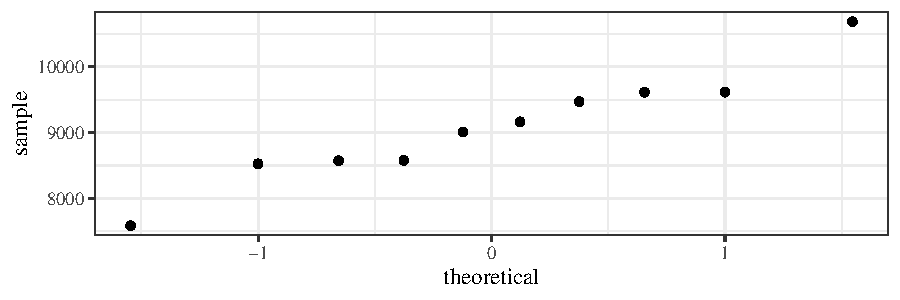
\includegraphics{stat305_hw10-003}

    Notice that the normal plot of these data given above is reasonably linear. It may thus be sensible to suppose that breaking strengths for generic towels of this type (as measured by the students) are adequately modeled as normal. Under this assumption,
          \begin{enumerate}
            \item Make and interpret 95\% two-sided and one-sided confidence intervals (one-sided of the form $(\#, \infty)$) for the mean breaking strength of generic towels.[5 pts]
            \item Make and interpret 95\% two sided and one-sided prediction intervals for a single additional generic towel breaking strength. For the one-sided interval, give the lower prediction bound. [5 pts]
          \end{enumerate}
    

%           
%  \item  Metro Construction Analytics (MCA) is a firm specializing in analyzing data for major construction companies. 
% One of their clients is interested in determining the true average time it takes to build a specific style of a three bedroom, two-and-a-half bathroom home, called an Average Design Rural Occupant Construction (or ADROC).
% The client provides MCA with the number of days from start of construction to completion for 40 houses in the ADROC style. 
% The client also promises MCA that they know the standard deviation for construction of such a house is 80 days.
% The 40 construction times are reported below and have an average of 193.8 days.
%   \begin{table}[h]
%      \centering
%      \label{tab:label}
%      \begin{tabular}{rrrrrrrrrr}
%         192 & 188 & 208 & 300 & 191 & 140 & 185 & 242 & 176 & 238 \\
%         124 & 184 & 171 & 181 & 198 & 161 & 221 & 171 & 178 & 156 \\
%         225 & 193 & 178 & 163 & 183 & 230 & 210 & 179 & 138 & 159 \\
%         296 & 146 & 233 & 239 & 179 & 304 & 163 & 138 & 184 & 207 \\
%      \end{tabular}
%   \end{table}
%   In this problem, let $\mu$ represent the true average time it takes to build an ADROC style home.
% 
%   \begin{enumerate}
%      \item Provide a 90\% confidence interval for the true mean $\mu$. [5 pts]
%      \item Provide a 95\% confidence interval for the true mean $\mu$. [5 pts]
%      \item Provide a 99\% confidence interval for the true mean $\mu$. [5 pts]
%   \end{enumerate}
%    
 
Total: 90 pts



\end{document}
